\documentclass[10pt]{beamer}
\usetheme[
%%% option passed to the outer theme
%    progressstyle=fixedCircCnt,   % fixedCircCnt, movingCircCnt (moving is deault)
  ]{Feather}
  
% If you want to change the colors of the various elements in the theme, edit and uncomment the following lines

% Change the bar colors:
%\setbeamercolor{Feather}{fg=red!20,bg=red}

% Change the color of the structural elements:
%\setbeamercolor{structure}{fg=red}

% Change the frame title text color:
%\setbeamercolor{frametitle}{fg=blue}

% Change the normal text color background:
%\setbeamercolor{normal text}{fg=black,bg=gray!10}

%-------------------------------------------------------
% INCLUDE PACKAGES
%-------------------------------------------------------

\usepackage[utf8]{inputenc}
\usepackage[english]{babel}
\usepackage[T1]{fontenc}
\usepackage{helvet}

%-------------------------------------------------------
% DEFFINING AND REDEFINING COMMANDS
%-------------------------------------------------------

% colored hyperlinks
\newcommand{\chref}[2]{
  \href{#1}{{\usebeamercolor[bg]{Feather}#2}}
}

%-------------------------------------------------------
% INFORMATION IN THE TITLE PAGE
%-------------------------------------------------------

\title[] % [] is optional - is placed on the bottom of the sidebar on every slide
{ % is placed on the title page
      \textbf{ATORES NA REDE DE CUIDADO A HIPERTENSOS E DIABÉTICOS}
}

\subtitle[The Feather Beamer Theme]
{
      \textbf{ANÁLISE DE REDE SOCIAL DE UMA ENFERMEIRA DA ESF DE UM MUNICÍPIO DE PEQUENO PORTE}
}

\author[Alexandra da Silva Lima Vieira]
{      Alexandra da Silva Lima Vieira \\
      {\ttfamily lima.alexandra@gmail.com}\\
      Orientadora: Profa. Dra. Maria Rocineide Ferreira da Silva \\
      {\ttfamily rocineideferreira@gmail.com}
}


\institute[]
{
	Centro de Ciências da Saúde - Enfermagem\\
      Universidade Estadual do Ceará\\
  
  %there must be an empty line above this line - otherwise some unwanted space is added between the university and the country (I do not know why;( )
}

\date{\today}

%-------------------------------------------------------
% THE BODY OF THE PRESENTATION
%-------------------------------------------------------

\begin{document}

%-------------------------------------------------------
% THE TITLEPAGE
%-------------------------------------------------------

{\1% % this is the name of the PDF file for the background
\begin{frame}[plain,noframenumbering] % the plain option removes the header from the title page, noframenumbering removes the numbering of this frame only
  \titlepage % call the title page information from above
\end{frame}}


\begin{frame}{Sumário}{}
%\tableofcontents
  \begin{itemize}
    \item Introdução
    \item Relevância
    \item Objetivo
    \item Metodologia
    \item Aspectos Éticos e Legais
    \item Análise de Dados
    \item Resultados e Discussão
    \item Conclusões e Trabalhos Futuros
    \item Referências
  \end{itemize}

\end{frame}

%-------------------------------------------------------
\section{Introdução}
%-------------------------------------------------------
\subsection{}
\begin{frame}{Introdução}{}
%-------------------------------------------------------

  \begin{itemize}
    \item Enfermeiro:  o articulador da equipe de saúde na AB, pois com
 suas competências gerenciais, tem no trabalho em equipe um caminho para a comunicação e
 contato entre os diferentes profissionais.
    \item Análise de Rede  Social (ARS): ferramenta que nos permite conhecer as interações entre qualquer  classe de indivíduos, partindo preferencialmente de dados qualitativos do que quantitativos.  (ALEJANDRO; NORMAN, 2005).
 	\item Na saúde, a ARS tem como foco a compreensão das relações entre
 os atores, ou seja, das relações entre os profissionais de diferentes categorias que participam do processo de comunicação, durante o cuidado prestado aos pacientes (SILVA et al., 2013).
 	\item Assim, questiona-se: como se configura a Rede Social para a linha de cuidado
 a pacientes hipertensos e diabéticos de uma enfermeira da ESF de um município de pequeno
 porte?
  \end{itemize}
\end{frame}

%-------------------------------------------------------
\section{Relevância}
%-------------------------------------------------------
\subsection{}
\begin{frame}{Relevância}{}
%-------------------------------------------------------

\begin{block}{}
  \begin{itemize}
    \item Compreender melhor os elementos que permitem a este profissional configurar, participar e/ou liderar, explicita ou tacitamente as redes sociais visando responder às demandas e necessidades cotidianas dos usuários hipertensos e diabéticos.
  \end{itemize}
\end{block}
\end{frame}

%-------------------------------------------------------
\section{Objetivo}
%-------------------------------------------------------
\subsection{}
\begin{frame}{Objetivo}{}
%-------------------------------------------------------

\begin{block}{}
  \begin{itemize}
    \item Analisar a rede social de uma enfermeira da Estratégia Saúde da Família de Icapuí-Ce para hipertensos e diabéticos.
  \end{itemize}
\end{block}
\end{frame}
     

%-------------------------------------------------------
\section{Metodologia}
%-------------------------------------------------------
\subsection{}
\begin{frame}{Metodologia}{}
%-------------------------------------------------------
  \begin{itemize}
    \item Tipo de Estudo: Estudo de caso de abordagem qualitativa e exploratória.
    \item Cenário e participantes da pesquisa.
    \begin{itemize}
    		\item Saúde de Icapuí: 8 equipes de ESF, NASF residente, hospital municipal, CAPS geral.
            \item Participantes da pesquisa: Trabalhadores da saúde acionados a partir da enfermeira da UBS de Barreira com diferentes vínculos com o município ou com sua rede de assistência. 
    \end{itemize}
  \end{itemize}
\end{frame}

%-------------------------------------------------------
\section{}
%-------------------------------------------------------
\subsection{}
\begin{frame}{Metodologia (Cont.)}{Coleta de dados}
%-------------------------------------------------------
  \begin{itemize}
	\item Questionamentos: 
	\begin{itemize}
    	\item Formação dos participantes, tempo de atividade no Sistema de Saúde municipal, percepção do sistema de referência e contra-referência municipal a hipertensos e diabéticos, situações de ativação de outros atores para a continuidade do cuidado a esses pacientes e as cinco pessoas que elas julgassem serem as mais ativadas por elas para suas redes sociais no que tange ao desempenho de suas ações de cuidado.
     \end{itemize}
     \item  Enfermeira UBS de Barreira aciona 5 atores e cada um desses 5 aciona mais 5 de suas respectivas redes 
  \end{itemize}
\end{frame}

%-------------------------------------------------------
\section{Aspectos Éticos e Legais}
%-------------------------------------------------------
\subsection{}
\begin{frame}{Aspectos Éticos e Legais}{}
%-------------------------------------------------------
  \begin{itemize}
	\item Comitê de Ética e Pesquisa 
    \begin{itemize}
    	\item Projeto: Redes sociais no trabalho de enfermeiros da Atenção Básica: um estudo em municípios do Rio de Janeiro e Ceará.
		\item Comitê de Ética em Pesquisa (CEP) da Universidade Estadual do Ceará, Resolução 466/2012 do Conselho Nacional de Saúde (CNS).
    \end{itemize}
    \item Assinatura do TCLE
    \begin{itemize}
		\item Informação sobre a pesquisa e o instrumento, garantia de sigilo e uso de dados para a pesquisa
    \end{itemize}
  \end{itemize}
\end{frame}


%-------------------------------------------------------
\section{Análise de Dados}
%-------------------------------------------------------
\subsection{}
\begin{frame}{Análise de Dados}{}
%-------------------------------------------------------
  \begin{itemize}
	\item Análise de Redes Sociais:
    \begin{itemize}
    	\item O uso de análise de redes sociais possibilita coletar informações relevantes
 sobre a estrutura de um grupo, sendo possível, identificar as posições ocupadas pelos indivíduos, bem como identificar o cerne das relações criadas ao redor de cada um.(STANLEY;
 KATHERINE, 1994)
    \end{itemize}
    \item Utilizados softwares UCINET versão 6.18 e Netdraw
    \item Grafo gerado:
    \begin{itemize}
    	\item Os atores sociais citados tiveram os nomes decodificados para a análise dos dados no software.
        \item O grafo gerado foi analisado visando identificar quais foram os profissionais mais acessados pela enfermeira cuja rede foi inicialmente analisada, como também a localização da mesma profissional dentro da rede que se construiu a partir dos atores posteriormente citados.
    \end{itemize}
  \end{itemize}
\end{frame}

%-------------------------------------------------------
\section{Resultados e Discussão}
%-------------------------------------------------------
\subsection{}
\begin{frame}{Resultados e Discussão}{}
%-------------------------------------------------------
  \begin{itemize}
	\item Considerando que a rede pesquisada não contempla todas as relações possíveis e existentes de cada pessoa entrevistada, mas somente um recorte viável de analisar: número limitado de atores, conexões e métricas.
    \item Exemplos de notação de representação dos atores [Profissão][Identificador] [Área de Atuação].
    \begin{itemize}
    	\item E0
        \item E2 [H]
        \item N0 [R]
    \end{itemize}
  \end{itemize}
\end{frame}

%-------------------------------------------------------
\section{}
%-------------------------------------------------------https://www.overleaf.com/3005378jkkgqn#
\subsection{}
\begin{frame}{Resultados e Discussão (Cont.)}{}
%-------------------------------------------------------
\begin{figure}[htbp]
\centering
 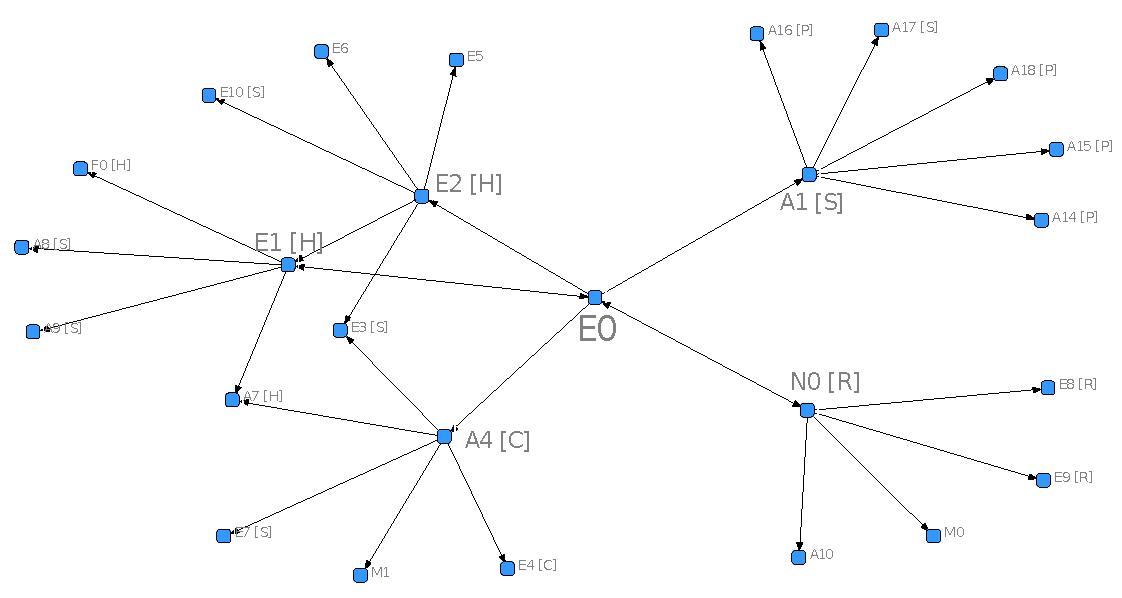
\includegraphics[width=\textwidth]{figuras/grafo.pdf}
 \caption{Representação da rede social utilizada neste trabalho.}
\label{fig:grafos}
\end{figure}
\end{frame}


%-------------------------------------------------------
\section{}
%-------------------------------------------------------
\subsection{}
\begin{frame}{Resultados e Discussão (Cont.)}{}
%-------------------------------------------------------
  \begin{itemize}
    \item Medidas e Discursos:
    \begin{itemize}
    	\item Densidade: relação entre o número de enlaces existentes e o número de enlaces possíveis. Tal métrica exibe a taxa de conectividade da rede. 
	\item O valor de densidade encontrado foi de 4,61\% (baixa densidade) o que pode denotar a existência de alguma dificuldade na resolução de problemas em grupo
	\item Motivos de baixa densidade: Os atores não conseguem se identificar como participantes de um grupo maior e podem demonstrar certa dificuldade de relacionamento. Tal situação pode acarretar pouca cooperatividade entres os atores envolvidos, podendo até mesmo existir apatia na resolução de problemas, gerando conflitos.(HANNEMAN;HANNEMAN, 2001)
    \end{itemize}
  \end{itemize}
  No estudo, atores se localizam em diferentes locais de trabalho, o que dificulta o desenvolvimento da comunicação, além disso, as motivações pessoais para a denominação de certos atores devem ser levada em consideração.
\end{frame}

%-------------------------------------------------------
\section{}
%-------------------------------------------------------
\subsection{}
\begin{frame}{Resultados e Discussão (Cont.)}{}
%-------------------------------------------------------
  \begin{itemize}
    \item Grau de Centralidade:
    \begin{itemize}
    	\item número de ligações que entram e que saem de um ator. 
	\item Através dele são identificados os atores principais da rede.
    \end{itemize}
  \end{itemize}
\begin{figure}[htbp]
\centering
 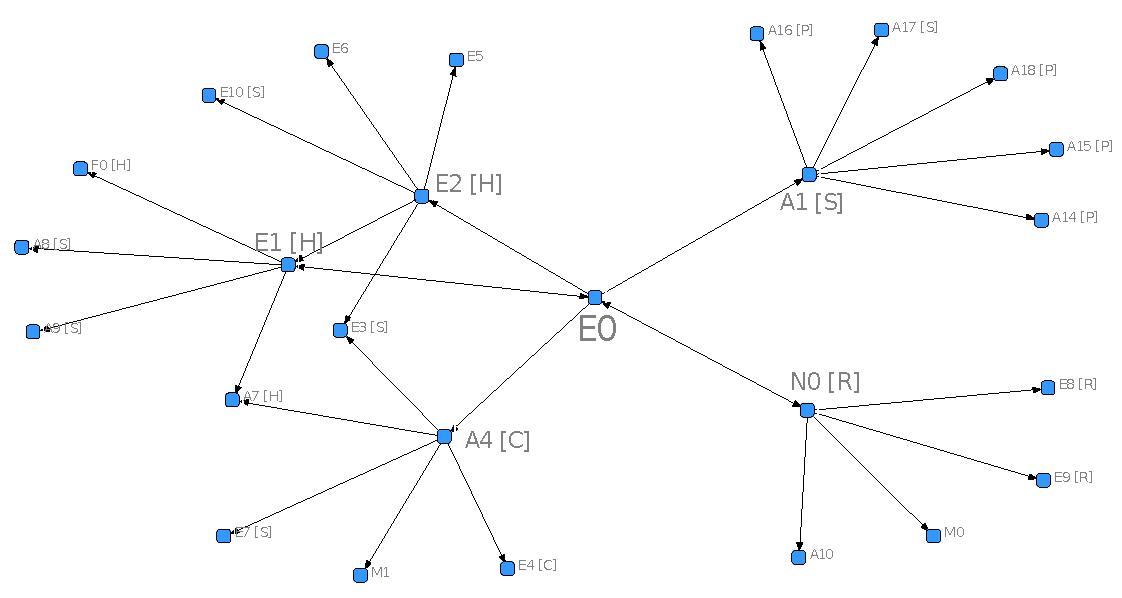
\includegraphics[width=.7\textwidth]{figuras/grafo.pdf}
 \caption{Representação da rede social utilizada neste trabalho.}
\label{fig:grafos}
\end{figure}
  Principais atores da rede são E0, E1[H],A7[H] e E3[S] pois cada um possui Grau de Entrada Normalizada de 0,8 (mais requisitados)
\end{frame}

%-------------------------------------------------------
\section{}
%-------------------------------------------------------
\subsection{}
\begin{frame}{Resultados e Discussão (Cont.)}{}
%-------------------------------------------------------
  \begin{itemize}
    \item E0 como ator central:
    \begin{itemize}
    	\item Enfermeira foi uma das primeiras enfermeiras a integrar a ESF. Está no quadro de funcionários do município como enfermeira desde o fim da graduação tendo passado também pelo Hospital Municipal, integrando a equipe assistencial.
	\item ``Esse mesmo tempo, que quando eu me formei eu vim pra cá, e fiquei trabalhando aqui em Barreiras e mais em outra área, a gente conjugava duas unidade de saúde, quando iniciou a formação do PSF do município, então não tinha muito profissional na época, então a gente se dividia em duas equipes, com o passar do tempo que a gente foi... Eu to aqui só em Barreiras mesmo, esses vinte anos, mas eu sempre dividi até o ano passado dividi com outra unidade de saúde.'' (E0)
    \end{itemize}
  \end{itemize}
E0 teve a oportunidade de servir como referência a outros profissionais que adentraram no programa posteriormente. Seu período como plantonista no hospital, também proporcionou a ela o desenvolvimento de outras relações com outros profissionais, como E1[H] e E2[H].
\end{frame}

%-------------------------------------------------------
\section{}
%-------------------------------------------------------
\subsection{}
\begin{frame}{Resultados e Discussão (Cont.)}{}
%-------------------------------------------------------
  \begin{itemize}
    \item E1[H] como ator central: 
    \begin{itemize}
    	\item coordenador do serviço de enfermagem do hospital, além de enfermeiro plantonista. E1[H] cita E0 e é citado por esta, pois desenvolveram um vínculo devido ao período em que trabalharam juntos no hospital. É citado também por E2[H].
	\item ``(...) eu já falei e to repetindo porque eu realmente to emocionado, ela acompanhou o meu trajeto, é...da minha profissão como eu falei anteriormente, desde o comecinho e me acompanha até hoje, e hoje a gente é colega de trabalho, e ela sempre me procura quando precisa, e isso faz um vínculo muito forte, que eu não quero que quebre nunca.'' (E1[H])
    \end{itemize}
  \end{itemize}
\end{frame}

%-------------------------------------------------------
\section{}
%-------------------------------------------------------
\subsection{}
\begin{frame}{Resultados e Discussão (Cont.)}{}
%-------------------------------------------------------
  \begin{itemize}
    \item A7[H] como ator central:
    \begin{itemize}
    	\item Diretora administrativa do hospital.
    	\item Citada por E1[H] e A4[C].
    	\item Para E1[H] uma pessoa procurada para resolver problemas relacionados ao atendimento hospitalar a esses paciente e outras questões de ordem gerencial.
    	\item Para A4[C], A7[H] administra conflitos, facilitando a acesso do usuário.
	\item ``(...)e a diretora do hospital, porque às vezes o médico que ta de plantão, não conhece o trabalho do CAPS, não conhece o paciente, se nega a fazer, então a diretora vai lá e aí ajeita tudo, e dá um jeito de contornar a situação né, paciente não ficar sem atendimento.'' (A4[C])
    \end{itemize}
  \end{itemize}
\end{frame}

%-------------------------------------------------------
\section{}
%-------------------------------------------------------
\subsection{}
\begin{frame}{Resultados e Discussão (Cont.)}{}
%-------------------------------------------------------
  \begin{itemize}
    \item E3[S] como ator central:
    \begin{itemize}
    	\item Coordenador da AB do município.
    	\item Citado por A4[C] e E2[H].
    	\item O cargo de gestão facilita o contato entre os diversos profissionais, realiza pactuações e articulações entre serviço e comunidade:
	\item ``(...)às vezes acontece dum médico se recusar, mas aí a gente vai e comunica a secretaria de saúde, e aí E3[S], ele é o coordenador, vai lá e conversa passa o caso pra ele, e aí tudo se resolve.
'' (A4[C])
    \end{itemize}
  \end{itemize}
\end{frame}

%-------------------------------------------------------
\section{}
%-------------------------------------------------------
\subsection{}
\begin{frame}{Resultados e Discussão (Cont.)}{Grau de proximidade e Grau de Intermediação}
%-------------------------------------------------------
  \begin{itemize}
    \item Grau de proximidade: a capacidade de um ator se ligar a todos os outros atores de uma rede, ou seja, quanto menor a distância entre um ator e outro, maior será seu grau de proximidade.
    \item Grau de intermediação: mostra a capacidade que um ator possui de intermediar a  comunicação entre pares de atores da rede. Sua importância se dá, pois, através de atores que possuem alto grau de intermediação que as informações são propagadas para diversos outros atores.
    \item Atores E0, A1[S], E1[H], N0[R], A4[C] e E2[H] - maiores Graus de Proximidade atores E0, A1[S] e N0[R] -possuem maiores Graus de Intermediação.
    \item E0 possui maior grau de intermediação pois a rede foi construída a partir dela. Mas destaca-se a mesma medida de A1[S]. 
    \item A1[S] é responsável pela distribuição de um grande número de informações na rede. 
    \item Outros achados: Foram citados atores residentes, mostrando a importância desse processo formativo.
    \end{itemize}
\end{frame}


%-------------------------------------------------------
\section{}
%-------------------------------------------------------
\subsection{}
\begin{frame}{Conclusões e Trabalhos Futuros}{}
%-------------------------------------------------------
  \begin{itemize}
    \item Atores enfermeiros e outros profissionais de enfermagem na rede.
    \item Vínculos formais e informais na qualidade dos enlaces expandindo a rede.
    \item A ARS para estudos futuros e a entrevista como instrumento de coleta.
    \end{itemize}
\end{frame}

%-------------------------------------------------------
\section{}
%-------------------------------------------------------
\subsection{}
\begin{frame}{Referências}{}
%-------------------------------------------------------
ALEJANDRO, V.; NORMAN, A. G. Manual introdutório à análise de redes sociais. UAEM–
Universidad Autonoma Del Estado de Mexico, 2005.

HANNEMAN, R. A.; HANNEMAN, R. Centralidad y poder. HANNEMAN, RA Introducción
a los métodos del análisis de redes sociáles. Departamento de Sociología de la Universidad
de California Riverside, 2002a. cap, v. 6, 2001

SILVA, A. S. da; AVELAR, A. B. A.; FARINA, M. C. Transferência intra-hospitalar de pacientes:
Uma aplicação da análise de redes sociais. XXVII Encontro da ANPAD, 2013.

STANLEY, W.; KATHERINE, F. Social network analysis. Theory and applications. [S.l.]:
Cambridge, Cambridge University Press, 1994.
\end{frame}




{\1
\begin{frame}[plain,noframenumbering]
  \finalpage{Obrigada! Perguntas?}
\end{frame}}

\end{document}